\subsection{High Level Design}

Figure \ref{figures:artemis_ssps} depicts the high-level design and the components involved in the extension module for SSPS on Apache ActiveMQ Artemis. 

Since the SSPS was designed using the MQTT protocol, the extension is also designed only to work with MQTT protocol. The user applications communicate using the MQTT protocol. All the incoming MQTT packets are intercepted by the MQTT interceptor. The MQTT interceptor sends the packets to the Sampling Broker through JMS, which is described in detail in next section. Sampling Broker works in parallel with Artemis Server performing dictionary sampling, maintenance, and distribution across the subscribers and publishers. 
\makeatletter
\setlength{\intextsep}{20pt}
\makeatother

\begin{figure}[h!]
\centering
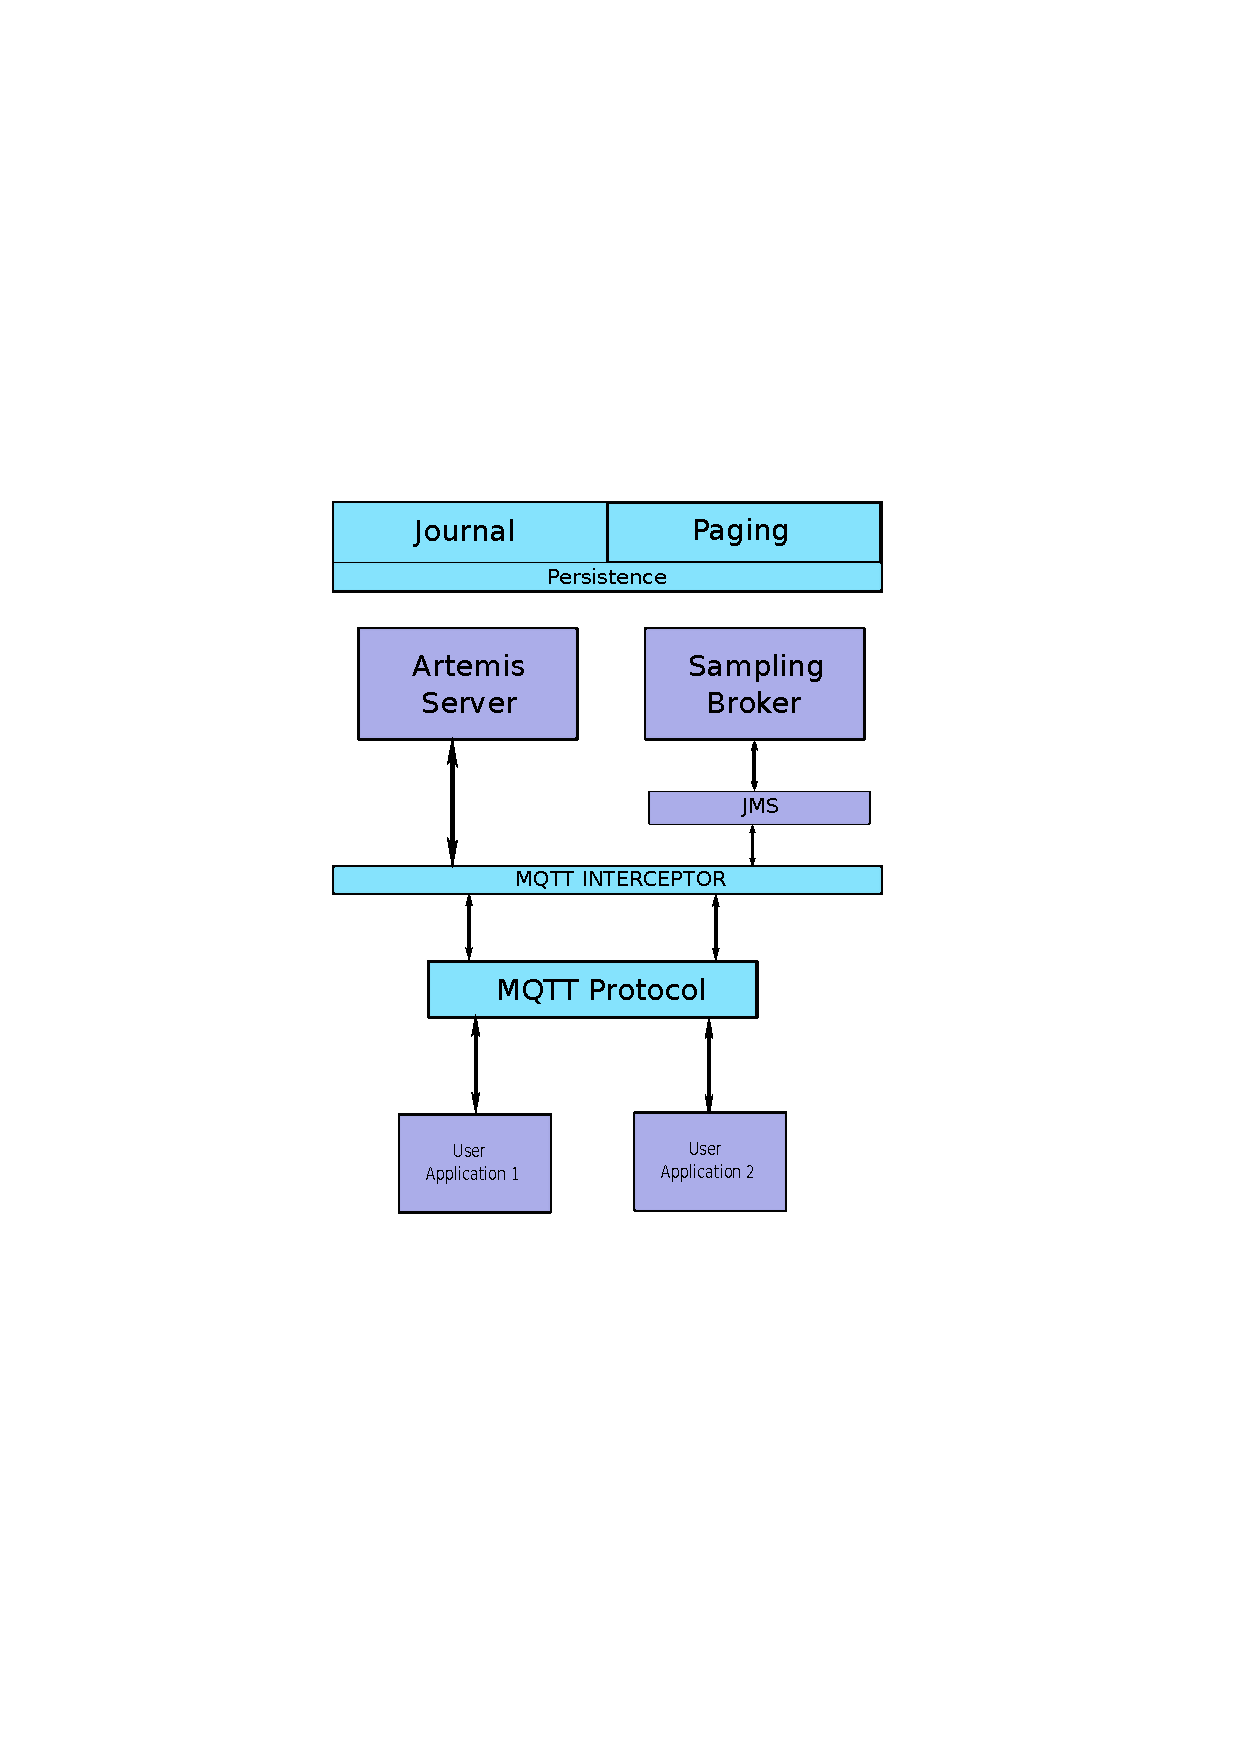
\includegraphics[keepaspectratio, width=1.1\textwidth, trim={3cm 8cm 0 8cm},clip]{artemis_ssps.pdf}
\caption{SSPS for Apache ActiveMQ Artemis High Level Design}\label{figures:artemis_ssps}
\end{figure}

The high-performance journal of Apache ActiveMQ Artemis is used for persistence. Both messages and dictionaries are persisted using the journals to handle failover. Paging comes into the picture in case of low memory situations.